\documentclass[a4paper,12pt]{article}

% Packages
\usepackage{amsmath}         % Math
\usepackage{amsfonts}        % Fonts
\usepackage{amssymb}         % Symbols
\usepackage{graphicx}        % Graphics
\usepackage{geometry}        % Page layout
\usepackage{tikz}            % For drawing the plot
\usepackage{hyperref}        % Links and references (подключаем в конце!)
\usepackage[T2A]{fontenc}    % Кодировка шрифтов
\usepackage[utf8]{inputenc}  % Кодировка входного файла (UTF-8) % Русский язык

% Page layout settings
\geometry{top=1in, bottom=1in, left=1in, right=1in}

\title{Formal Description for the Transformation of Planar Coordinates into Spherical Coordinates and Further Computation of Coordinates}
\author{by DanLyss}
\date{\today}

\begin{document}

% Title page
\maketitle

% Abstract
\begin{abstract}
   The goal of this paper is to provide all necessary formulas for the AstroNavigation project, as well as their derivation. Some algorithms for solving non-linear systems are also suggested.
\end{abstract}

% Sections and content
\section{Transformation of Planar Coordinates on the Picture to Spherical Coordinates}

\begin{figure}[h]
    \centering
 
    \begin{tikzpicture}
        \draw[->] (-2.8,0) -- (2.8,0) node[right] {$x$};
        \draw[->] (0,-2.8) -- (0,2.8) node[above] {$y$};
        \filldraw (1,2) circle (2pt) node[above right] {$(x_0, y_0)$};
        \filldraw (-2,-1) circle (2pt) node[below left] {$(x_1, y_1)$};
        \draw[thick] (0,0) -- (1,2);
        \draw[thick] (0,0) -- (-2,-1);

        \draw[->] (0.5,0) arc (0:63.43:0.5) node[midway, right] {$\theta_0$};
        \draw[->] (-0.5,0) arc (180:206.57:0.5) node[midway, left] {$\theta_1$};

        \draw[<->] (-4,-3.3) -- (4,-3.3) node[midway, below] {$L$};

        \draw[<->] (4.3,-3) -- (4.3,3) node[midway, right] {$H$};
    \end{tikzpicture}

    \caption{Projection of part of the celestial sphere on the tangent plane}
    \label{fig:coordinate_plane}
\end{figure}
For each star on the picture we measure pair of coordinates \((x_0, y_0)\). Size of the picture is \(L\)\texttimes \(H\). Units of measurements are pixels. Let's also draw celestial sphere to show where coordinate plane is located

\begin{center}
    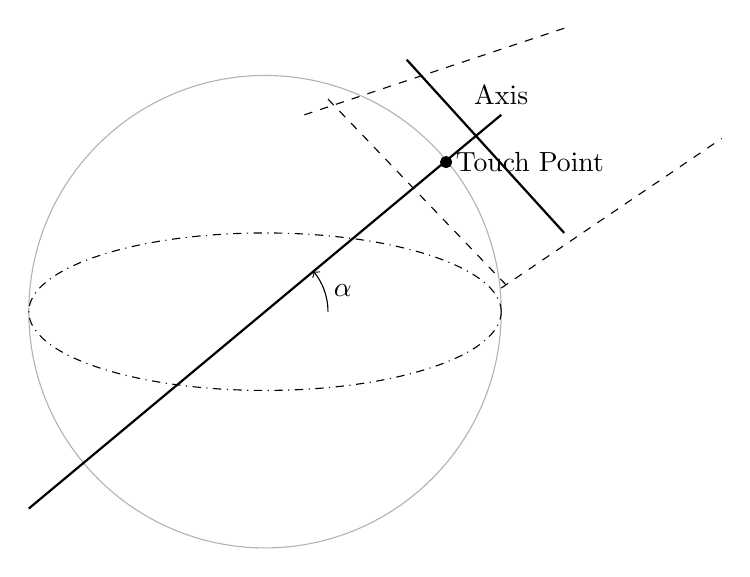
\begin{tikzpicture}

        \draw[opacity=0.3] (0,0) circle (3);

        \draw[dash dot] (0,0) ellipse (3 and 1);

        \draw[thick] (-3,-2.5) -- (3,2.5) node[above] {Axis};

        \draw[->] (0.8,0) arc (0:40:0.8) node[midway, right] {$\alpha$};

        \filldraw (2.3,1.9) circle (2pt) node[right] {Touch Point};

        \begin{scope}
          \draw[dashed] (0.8,2.7) -- (3.1,0.3);
            \draw[dashed] (0.5,2.5) -- (3.8,3.6);
            \draw[dashed] (3,0.3) -- (5.8,2.2);
            \draw[thick] (1.8,3.2) -- (3.8,1);
        \end{scope}

    \end{tikzpicture}
\end{center}
(Now, I am tired of drawing pictures with LaTeX so will insert hand drawen images)

We have the following picture taken:
\par
    \centering
    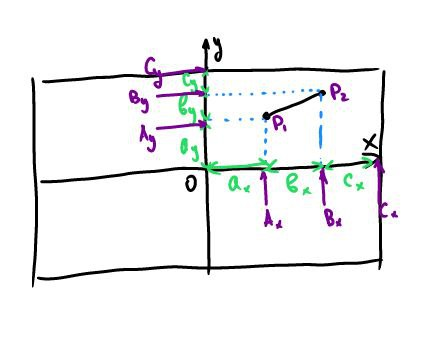
\includegraphics[width=0.5\textwidth]{pic_pars.jpg}

\par \par
Here, \(P_1\) and \(P_2\) are some two stars, \(a_x, b_x, c_x, a_y, b_y, c_y\) - lengths in pixels.
\par
Consider axis y. Let's see how it actually corresponds to the sky
    \centering
    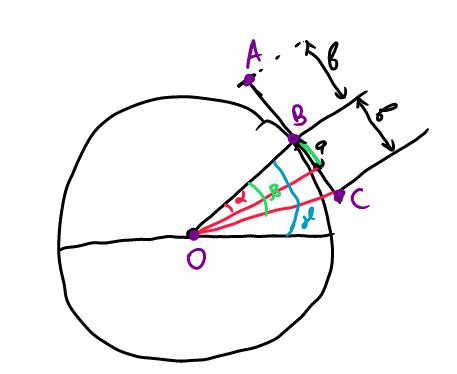
\includegraphics[width=0.5\textwidth]{size_if_know.jpg}
\par
Angle \(\gamma\) is the height of the center of the picture above the horizon that is taken from hyroscope measurements. Suppose, that we already found \(\beta\) - angular horizontal size of the picture. \(a, b\) could be directly measured from the picture. Then 
\begin{equation}
\frac{a}{tan(\alpha)} = \frac{b}{tan(\beta)} \Rightarrow \alpha = arctan( \frac{a \cdot tan(\beta)}{b})
 \end{equation}
However, we don't know \(\beta\). But, given two stars \(P_1\) and \(P_2\), we can measure \(a_x, b_x, c_x, a_y, b_y, c_y\). Believeing in spherical projection, lets solve for horizontal angular size.
\par
We have 
\par
   \centering
    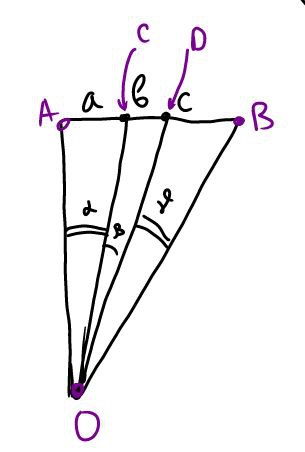
\includegraphics[width=0.5\textwidth]{solving_triangle.jpg}
\par
Here, \(a\) is \(a_y\), \(b\) is \(b_y\), \(c\) is \(c_y\). \(\beta\) is angular distance between stars \(P_1\) and \(P_2\) projected on \(x\)-axis. Since after projection angles doesn't change, one may write
\begin{equation}
\beta = \delta \cdot \frac{\sqrt{b_x^2 + b_y ^ 2}}{b_x}
\end{equation}
where \(\delta\) is angular distance between \(P_1\) and \(P_2\).
\par
To solve the triangle for \(\alpha + \beta + \gamma\), we write
\begin{equation}
    \begin{split}
        \frac{a}{\tan(\alpha)} &= \frac{a+b}{\tan(\alpha + \beta)} \Rightarrow 
        a \cdot \frac{\tan(\alpha) + \tan(\beta)}{1 - \tan(\alpha) \cdot \tan(\beta)} =
        (a+b) \cdot \tan(\alpha) \Rightarrow \\
        &-\tan^2(\alpha) \cdot (a + b) \cdot \tan(\beta) + \tan(\alpha) \cdot b - \tan(\beta) \cdot a = 0
    \end{split}
\end{equation}
Solving quadratic equation, we obtain
\begin{equation}
\tan(\alpha) = \frac{b \pm \sqrt{(b ^ 2 - 4 (a + b) \cdot \tan(\beta) ^ 2 \cdot a}}{2 \cdot (a + b) \cdot \tan(\beta)}
\end{equation}
From here, we get two possible values for \(\alpha\). And it makes sense after looking at the picture below
\par
   \centering
    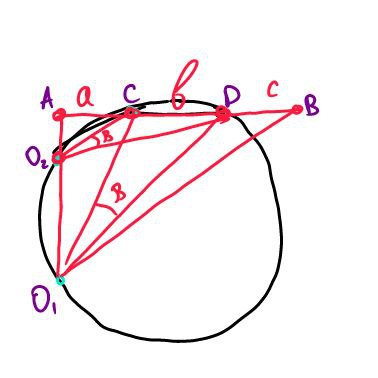
\includegraphics[width=0.5\textwidth]{2_cases.jpg}
\par
Indeed, there are two points \(O_1\) and \(O_2\) satisfying this equation.
To reduce this uncertainty, we suggest to perform these calculations for N pairs of stars and take the most often root
Ending up calculations
\begin{equation}
    \frac{a + b + c}{\tan(\alpha + \beta + \gamma)} = \frac{a}{\tan(\alpha)}
    \Rightarrow (\alpha + \beta + \gamma) = \arctan\left(\frac{(a + b + c) \cdot \tan(\alpha)}{a}\right)
\end{equation}
So, we managed to find angular vertical size of the picture. Same shall be performed for horizontal angular size.
Then, applying formula (1) one can obtain actual height above the horizon of the star. Regariding the azimuth, it can be computed up to the constant in the same manner. There is a little trick to show that change of angle along x - axis corresponds to azimuth change, which is left to a curious reader
\par \par
\section{Coordinates of location from star coordinates}
\subsection{Latitude}
Now, as we managed to transform data from the picture to the actual spherical coordinates, lets consider a celestial sphere
\par
   \centering
    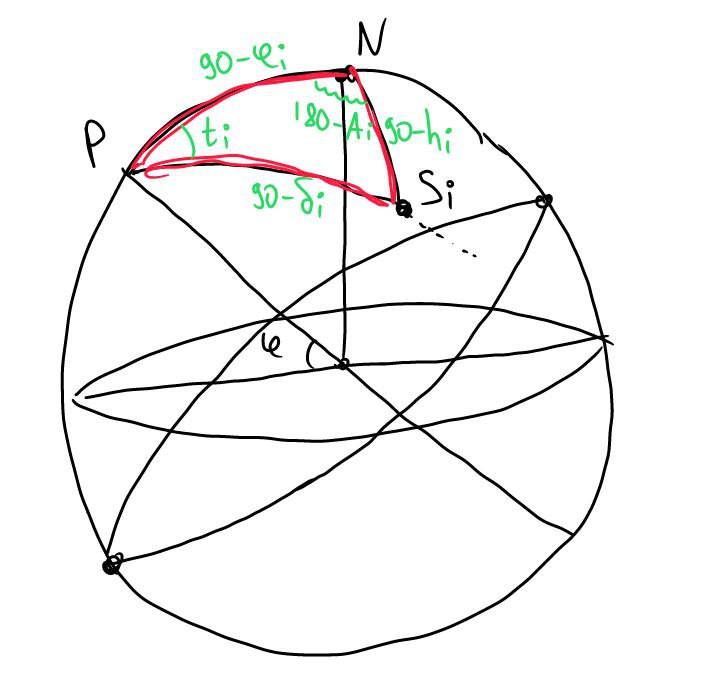
\includegraphics[width=0.5\textwidth]{spherical_geom.jpg}
\par
Here, \(S_i\) is some star, \(\delta_i\) - declination, \(h_i\) - height above the horizon, \(A_i\) - azimuth, \(\varphi_i\) (or just \(\varphi\)) is latitude, \(t_i\) - time angle
\par \par

The spherical law of cosines for three sides and one angle is:

\begin{equation}
\cos (90^\circ - \delta_i) = \cos(90^\circ - \varphi) \cos(90^\circ - h_i) + \sin(90^\circ - \varphi) \sin(90^\circ - h_i) \cos(180^\circ - A_i)
\end{equation}


Using trigonometric identities, we obtain
\begin{equation}
\sin (\delta_i) = \sin( \varphi) \sin( h_i )- \cos (\varphi_i )\cos (h_i) \cos (A_i)
\end{equation}
Lets take 2 stars, with \( i = 1\) and \( i = 2\)
\par
Then, 
\begin{equation}
\begin{aligned}
\sin (\delta_1) &= \sin( \varphi) \sin( h_1 ) - \cos (\varphi )\cos (h_1) \cos (A_1) \\
\sin (\delta_2) &= \sin( \varphi) \sin( h_2 ) - \cos (\varphi )\cos (h_2) \cos (A_2)
\end{aligned}
\end{equation}

The unknowns are \(\varphi\) and \(A_1\). \(A_2\) = \(A_1 + A_0\), where \(A_0\) - difference of azimuth was computed in first section fron the picture
Simplifying the system of 2 equations
\begin{equation}
\begin{aligned}
\sin (\delta_1) + \cos (\varphi )\cos (h_1) \cos (A_1)&= \sqrt{1 - \cos^2(\varphi)} \sin( h_1 )  \\
\sin (\delta_2) + \cos (\varphi )\cos (h_2) \cos (A_2) &= \sqrt{1 - \cos^2(\varphi)} \sin( h_2 )
\end{aligned}
\end{equation}
Then
\begin{equation}
\begin{aligned}
\sin^2 (\delta_1) + \cos^2 (\varphi )\cos ^2(h_1) \cos ^2(A_1) + 2 \cdot\sin (\delta_1) \cdot \cos (\varphi )\cos (h_1) \cos (A_1) &= (1 - \cos^2(\varphi) )\sin^2( h_1 )  \\
\sin ^2(\delta_2) + \cos^2 (\varphi )\cos^2 (h_2) \cos^2 (A_2) +  2 \cdot\sin (\delta_2) \cdot \cos (\varphi )\cos (h_2) \cos (A_2)  &= (1 - \cos^2(\varphi))\sin^2( h_2 )
\end{aligned}
\end{equation}
Then
\begin{equation}
\begin{aligned}
    \cos^2 (\varphi ) \big(\cos^2(h_1) \cos^2(A_1) + \sin^2(h_1)\big) 
    &+ \cos (\varphi ) \cdot \big(2 \sin (\delta_1) \cos (h_1) \cos (A_1)\big) \\
    &+ \sin^2(\delta_1) - \sin^2(h_1) = 0, \\
    \cos^2 (\varphi ) \big(\cos^2(h_2) \cos^2(A_1 + A_0) + \sin^2(h_2)\big) 
    &+ \cos (\varphi ) \cdot \big(2 \sin (\delta_2) \cos (h_2) \cos (A_1 + A_0)\big) \\
    &+ \sin^2(\delta_2) - \sin^2(h_2) = 0.
\end{aligned}
\end{equation}
We have 2 quadratic equations. Say, first one has roots \(x_{11}\), \(x_{12}\), and second one has roots \(x_{21}\), \(x_{22}\). At least one root of first equation is also a root of second equation. So we consider 4 cases. Let's talk in more details about case when, for example, \(x_{11}\) = \(x_{21}\). One may note, that \(x_{11}\) and \(x_{21}\) are actually functions of \(A_0\). So equating them, we can find \(A_0\), which will totally define \(\cos(\varphi)\). However, \(A_0\) won't be unique, so we will actually obtain \(N\) pairs of kind \((A_0, \varphi)\), which are valid candidates for solution. Same happens for all 4 cases.
\vspace{8 mm}

\par
 
After careful analysis of pairs of valid solutions one can note that there are not so many of them for each pair of stars (less than 10). So we suggest performing such analysis for \(N + 1\) stars, with fixed first star and varying second one. After this we obtain \(M\) possible pairs of answers \((A_0, \varphi)\). Here we now use the fact, that for true \(\varphi\), \(A_0\) shall coincide. This way, taking appropriately big \(N\) we perfectly reduce uncertainty and find right latitude

\subsection{Longitude}
Now, we again consider spherical triangle \(PNS_i\).
We write law of sines to find \(t_i\)
\begin{equation}
\frac{\sin(t_i)}{\cos(h_i)} = \frac{\sin(A_i)}{\cos(\delta_i)} 
\Rightarrow 
t_i = \arcsin\left(\frac{\cos(h_i) \cdot \sin(A_i)}{\cos(\delta_i)}\right)
\end{equation}
We actually want to find the exact local time at the point of location. Let's look at the following picture:
\par
   \centering
    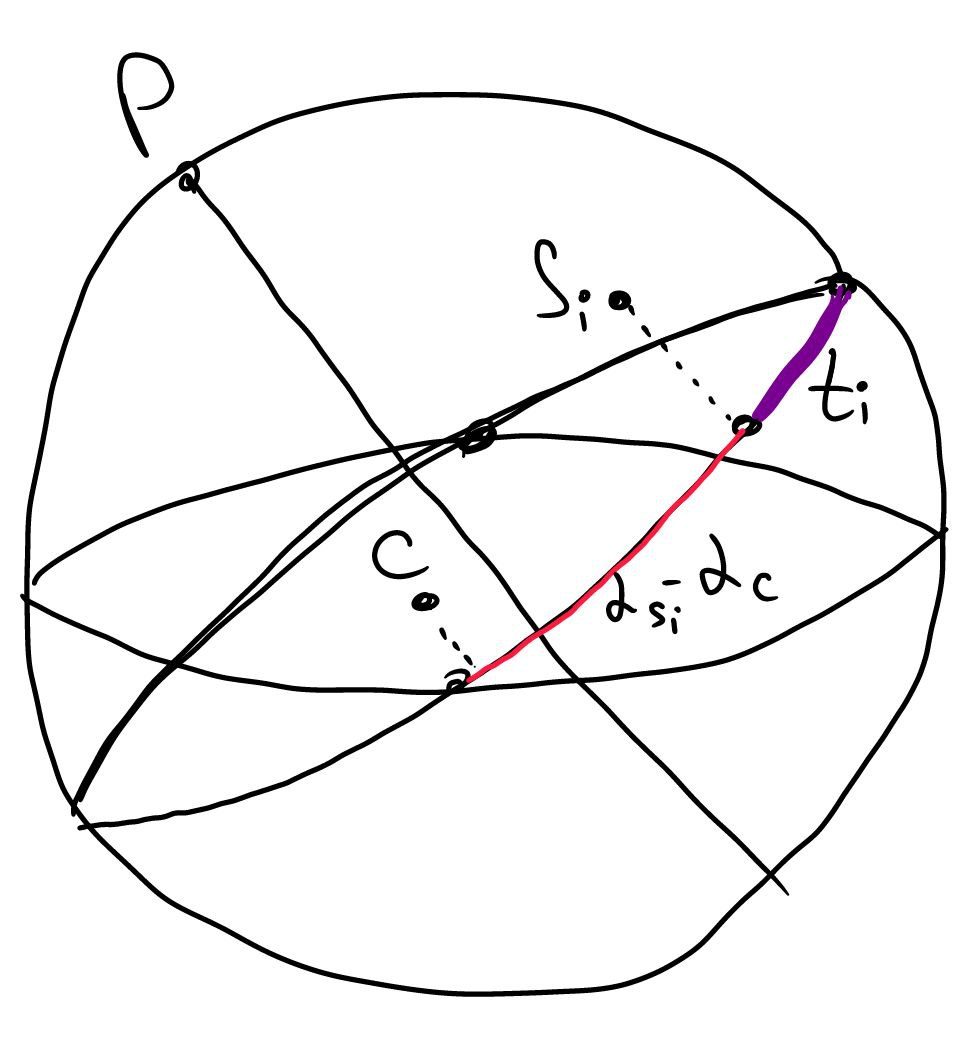
\includegraphics[width=0.5\textwidth]{time_det.jpg}
\par
Forgetting about time equation, Sun culminates at precisely 12 hours of local sun time (not time zone time)
Then local time right now, \(LT\), could be calculated as 
\begin{equation}
LT = 12^h + \frac{(t_i + \alpha_{S_i} - \alpha_c)}{360^\circ} \cdot 24^h
\end{equation}
Here, \(\alpha_{S_i}\) is right ascension of Sun and \(\alpha_c\) - right ascension of the star \(S_i\). We know everything, except Sun's right ascension. It shall be calculated. It's easy. We consider celestial equator and eclytpic plane
\par
   \centering
    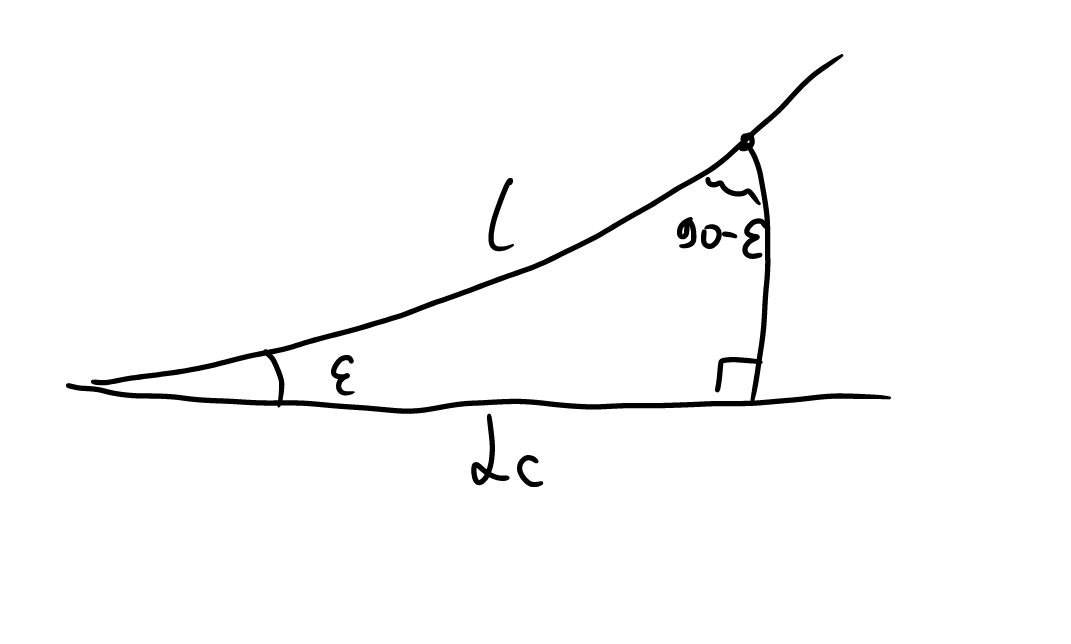
\includegraphics[width=0.5\textwidth]{SUN_RA.jpg}
\par
Applying, spherical law of sines, \(\alpha_c = \arcsin(\sin(l) \cdot \cos(\epsilon))\), \(l\) is angular length Sun traveled from spring equinox. One can easily count it knowing the time has passed since that date, and we know it pretty well since we know GMT time. \(\epsilon\) is angle between celestial equator and eclytpic plane. It's around \(23.44^\circ\).
\par 
\vspace{5mm}
Now, we also consider equation of time, \(ET\)(day), as a function of day. The exact form of time equation can be found in any astronomical literature, and here, I just note that it's needed to encounter for Earth axis inclination and Earth orbit being ellyptic.
The true sun local time then is 
\begin{equation}
TLT = LT - ET
\end{equation}
Now, if time at Greenwich is GMT, longitude is very easy to calculate
\begin{equation}
longitude = \frac{(TLT - GMT)}{24^h} \cdot 360^\circ
\end{equation}

AND WE ARE DONE
\end{document}